% =====================================================================
% Paper 16 - Multivariate Machine Learning for Cyber-Hygiene Anomaly
% Detection Across Active Directory, Endpoint, and Patch Telemetry.
% IEEE TNSM submission. Build with tectonic / XeLaTeX.
% Reproducibility: results/primary_v1/ (450 rows = 25 seeds x 3 conditions
% x 6 detectors; frozen on seeds 700-724). Run src/run_evaluation.py.
% =====================================================================
\documentclass[journal]{IEEEtran}

\usepackage{graphicx}
\usepackage{booktabs}
\usepackage{amsmath}
\usepackage{amssymb}
\usepackage{newtxtext,newtxmath}
\usepackage{hyperref}
\usepackage{xurl}
\usepackage{url}
\usepackage{array}

\graphicspath{{figures/}}

\title{Multivariate Machine Learning for Cyber-Hygiene Anomaly Detection\\
Across Active Directory, Endpoint, and Patch Telemetry}

\author{%
  \IEEEauthorblockN{Harshavardhan Malla}
  \IEEEauthorblockA{Independent Researcher\\
  Email: harshavardhanmalla75@gmail.com}%
}

\renewcommand{\textendash}{-}
\renewcommand{\textemdash}{-}
\usepackage{etoolbox}
\makeatletter
\patchcmd{\abstract}{---}{:\space}{}{}
\patchcmd{\IEEEkeywords}{---}{:\space}{}{}
\makeatother
\begin{document}
\maketitle

\begin{abstract}
Security operations teams watch endpoint fleets through three telemetry channels: Active
Directory, endpoint posture, and patch state. A compromised or misconfigured host appears as an
anomaly in this telemetry, and the operational question is whether multivariate machine-learning
anomaly detection earns its complexity over the per-signal threshold rules teams already run. We
answer with a pre-registered evaluation on a synthetic fleet of 1{,}500 hosts with a
12-dimensional hygiene telemetry vector, injecting two anomaly types: a single-channel anomaly
that crosses a per-feature threshold, and a cross-channel anomaly that keeps every feature
individually normal but breaks the correlation structure normal hosts exhibit. The answer is
conditional. On cross-channel anomalies a covariance-aware detector reaches average precision of
0.710 against 0.103 for the best per-feature rule (difference 0.607; 95\% BCa interval
$[0.598, 0.617]$). On single-channel anomalies the rule wins, 0.836 against 0.740 for the best
joint detector. The cross-channel advantage requires joint modeling, not aggregation: a
structure-blind exceedance count reaches 0.084. The choice of method is decisive: covariance-aware
(Mahalanobis, 0.710) and density-aware (Local Outlier Factor, 0.638) detectors see the violation,
while the axis-aligned Isolation Forest does not (0.105). On a fifty-fifty mixture the joint
detector still leads (0.702 against 0.473) but by a smaller margin (0.2285) than on cross-channel
anomalies alone. The deployable conclusion is a two-tier monitor: cheap rules for the obvious
single-channel spikes and a covariance- or density-aware detector for the subtle cross-channel
violations. The popular Isolation Forest is the wrong default for this anomaly class. We supply a
closed-form account: because the cross-channel anomaly preserves every marginal, per-feature and
axis-aligned detectors are provably at the prevalence floor while the expected squared Mahalanobis
distance separates the two covariance structures through the nonzero off-diagonal terms of the
inverse covariance, and this same structure is what a correlation-only adversarial evasion exploits.
\end{abstract}

\begin{IEEEkeywords}
anomaly detection, cyber hygiene, Active Directory, endpoint telemetry, Isolation Forest,
Local Outlier Factor, Mahalanobis distance, average precision, pre-registration
\end{IEEEkeywords}

\section{Introduction}
\IEEEPARstart{A}{security} operations team monitoring a large endpoint fleet sees three telemetry
channels. The first is Active Directory: privileged logon counts, security-group churn, the age of
stale administrative accounts, and the rate of failed authentications. The second is endpoint
posture: process-spawn anomalies, the fraction of unsigned binaries executed, configuration drift
from a hardened baseline, and host-firewall state. The third is patch state: aggregate patch debt,
days since the last successful patch, the presence of known-exploited
vulnerabilities~\cite{cisakev}, and the staleness of the host's own telemetry. Each channel is a
small bundle of numbers reported per host, and a fleet of a few thousand hosts produces a
continuous stream of these vectors. A host that has been compromised, misconfigured, or left to rot
shows up somewhere in this stream as an anomaly.

Teams already run per-signal threshold rules over these channels, because rules are cheap,
auditable, and easy to explain to an authorizing official. A rule fires when patch debt crosses a
line, when an account has been dormant past a deadline, or when too many unsigned binaries run in a
day. Rules of this kind catch the blatant cases and form the backbone of most operational hygiene
dashboards. The question this paper asks is whether multivariate machine-learning anomaly
detection~\cite{chandola2009anomaly,hodge2004survey} earns its additional complexity over those
rules, and if so, for which anomalies. The complexity is real: a joint detector must be fit,
maintained, explained, and trusted, and the anomaly-detection literature offers a confusing menu of
methods with no consensus default. A team that adopts the wrong method, or adopts any method where a
rule would have done, pays for the machinery without the benefit.

Our hypothesis, fixed before any evaluation, is that the answer depends on the geometric structure
of the anomaly rather than on a blanket judgment about machine learning. We distinguish two anomaly
types. A \emph{single-dimension anomaly} (SDA) is a threshold-crossing spike: one channel shifts
hard, patch debt jumps, an account count explodes, and a per-feature rule catches it by
construction. A \emph{cross-dimension anomaly} (CDA) is subtler. Every feature stays individually
within its normal range, so no per-feature rule fires, but the correlation structure that normal
hosts exhibit is broken. Normal hosts have channels that move together in characteristic ways; a
host whose channels have become mutually inconsistent, each plausible alone but jointly impossible,
is exactly the compromise-like case that per-feature inspection cannot see and a joint detector
should. If this distinction governs the outcome, the practical guidance is specific rather than
ideological: deploy multivariate detection for the subtle cross-channel cases and keep cheap rules
for the obvious single-channel ones.

We answer with a pre-registered simulation. A synthetic fleet of 1{,}500 hosts carries a
12-dimensional hygiene vector with documented within-channel correlation. Two anomaly types are
injected at fixed prevalence, and three evaluation conditions, single-channel only, cross-channel
only, and a fifty-fifty mixture, run on the same seeds. Six detectors compete: two per-feature rule
baselines and four joint detectors drawn from the standard anomaly-detection toolbox, all held at
fixed, untuned settings so that no detector gains from threshold or hyperparameter search.
Evaluation is threshold-free, by average precision~\cite{davis2006pr}, the appropriate metric for
ranking rare anomalies, with verdicts decided by the non-overlap of bias-corrected and accelerated
(BCa) bootstrap intervals~\cite{efron1987bca,efron1994introduction} rather than by significance
tests. The methodology follows the pre-registration discipline now standard in empirical software
engineering~\cite{wohlin2012experimentation}: hypotheses, thresholds, and the evaluation seed range
were locked before any evaluation result was inspected.

The contribution is fourfold.
\begin{itemize}
\item We show that the value of multivariate detection is \emph{conditional on anomaly structure},
not absolute. On cross-channel anomalies the best joint detector reaches average precision 0.710
against 0.103 for the best rule, a difference of 0.607 ($[0.598, 0.617]$); on single-channel
anomalies the rule wins, 0.836 against 0.740. Treating the two cases the same is the central error.
\item We show the cross-channel gain \emph{requires joint modeling, not aggregation}. A
structure-blind detector that merely counts per-feature exceedances reaches 0.084 on cross-channel
anomalies against 0.710 for the covariance-aware detector (difference 0.626). Summing marginal
alarms does not recover a correlation violation.
\item We show the \emph{choice of joint method is decisive}. Covariance-aware (Mahalanobis, 0.710)
and density-aware (Local Outlier Factor, 0.638) detectors see the violation; the axis-aligned
Isolation Forest (0.105) does not. A team that reaches for the most popular library detector would
wrongly conclude that machine learning does not help here.
\item We translate these into a deployable \emph{two-tier monitor}: cheap per-feature rules for the
obvious single-channel spikes and a covariance- or density-aware detector for the subtle
cross-channel violations, with the explicit warning that the default Isolation Forest is the wrong
tool for this anomaly class.
\end{itemize}

\section{Background and Related Work}

\subsection{Anomaly detection: taxonomy and surveys}
Anomaly detection is a mature field with two influential surveys that frame the present problem.
Chandola, Banerjee, and Kumar~\cite{chandola2009anomaly} organize the field by the nature of the
anomaly (point, contextual, and collective), by whether labels are available, and by output type
(label versus score), and they emphasize that the right method depends on the structure of the data
and of the anomaly rather than on a universal best algorithm. Hodge and Austin~\cite{hodge2004survey}
survey outlier-detection methodologies across statistics, machine learning, and neural networks and
make the same point from the statistical side: a method tuned to one kind of deviation can be blind
to another. Our two anomaly types are both point anomalies in their taxonomy, but they differ in
geometry: the single-channel anomaly is a large marginal deviation that any univariate method sees,
while the cross-channel anomaly is a deviation only in the joint distribution, invisible to any
method that inspects features one at a time. The surveys predict exactly the conditional outcome we
test, that the appropriate detector tracks the geometry of the anomaly.

\subsection{Density, boundary, and isolation methods}
The joint detectors we compare span the three dominant algorithmic families, and their differences
are the heart of the method-choice result. \emph{Density-based} methods score a point by how
isolated it is relative to the local density of its neighbors; the Local Outlier Factor (LOF) of
Breunig et al.~\cite{breunig2000lof} compares a point's local reachability density to that of its
neighbors, so a host that sits in a sparse region of the joint feature space, including a region
made sparse because its channels are mutually inconsistent, receives a high score. \emph{Boundary}
methods estimate the support of the normal distribution and flag points outside it; the One-Class
SVM of Sch\"olkopf et al.~\cite{scholkopf2001oneclass} fits a kernel boundary around the bulk of
the data, and its sensitivity to a correlation violation depends on whether the kernel and its
bandwidth resolve the relevant geometry. \emph{Isolation} methods isolate anomalies with random
recursive partitioning; the Isolation Forest of Liu, Ting, and Zhou~\cite{liu2008isolation} builds
trees of random \emph{axis-aligned} splits and scores a point by how few splits isolate it. The
axis-aligned construction is precisely why the Isolation Forest is expected to struggle on a
correlation violation: a split on a single feature cannot, by itself, express that two features have
become jointly inconsistent while each remains marginally normal. Outlier
ensembles~\cite{aggarwal2015outlier} combine such base detectors to hedge against any single
method's blind spots; we deliberately evaluate the base detectors individually, because the purpose
here is diagnostic, to expose which geometric assumption each family encodes, rather than to build
the strongest possible combined detector.

\subsection{Robust covariance and the Mahalanobis distance}
The parametric counterpart to these methods is the Mahalanobis distance under a fitted covariance,
the natural detector for a correlation-structure violation because it measures distance in the
metric induced by the inverse covariance. A host whose channels violate the normal correlation lies
far from the mean in this metric even when its per-feature values are unremarkable. The estimator
matters: an ordinary sample covariance is itself sensitive to the anomalies it is meant to detect,
so a robust covariance estimator is preferred. The Minimum Covariance Determinant estimator and its
fast algorithm of Rousseeuw and Van Driessen~\cite{rousseeuw1999mcd} fit the covariance to the
densest subset of the data, resisting contamination by outliers, and yield a Mahalanobis distance
that is robust to the very anomalies present at evaluation time. This is the detector we expect to
be best on cross-channel anomalies, because the cross-channel anomaly is, by construction, a
covariance violation, and a covariance-aware metric is the one that represents it.

\subsection{Why average precision for rare anomalies}
Anomalies are rare, and rare-event ranking must be scored by a metric that is not dominated by the
abundant normal class. Davis and Goadrich~\cite{davis2006pr} show that the precision-recall curve,
and its summary the average precision, is more informative than the ROC curve when the positive
class is rare, because ROC area can look deceptively high when there are many easy true negatives.
Average precision is also threshold-free: it summarizes the entire ranking a detector produces,
which is what an operations team consumes when it triages hosts in score order, so no detector gains
or loses from an arbitrary threshold choice. We therefore report average precision as the primary
metric for every detector and condition, and we evaluate the same ranking with no per-detector
threshold tuning.

\subsection{Federal hygiene-monitoring context}
Continuous fleet-wide hygiene monitoring is a federal expectation rather than an optional practice.
FIPS 199~\cite{fips199} sets the security categorization that determines the rigor a system owes,
the NIST SP 800-53 control catalog~\cite{nist80053} prescribes the configuration-management,
audit, and identity controls whose telemetry our channels stand in for, and SP
800-137~\cite{nist80137} establishes information security continuous monitoring as an ongoing
program. Sector policy such as the CJIS Security Policy~\cite{cjis2023} binds criminal-justice
agencies to comparable hygiene and audit requirements. None of these documents prescribes a
detection method; they require that hosts be watched, not how the watching ranks them. The present
study sits in exactly that gap, asking which detection method an agency that has accepted the
monitoring mandate should actually deploy, and for which anomalies. It complements our own line of
hygiene work: a reproducible benchmark for hygiene anomaly detection~\cite{paper3hygienebench} and
a study of hygiene-signal augmentation for vulnerability
prioritization~\cite{paper4hygieneprio}, both of which treat hygiene telemetry as a first-class
signal whose operational value must be measured rather than assumed.

\section{Method}
We model a single fleet over one snapshot and ask, for each detector and each anomaly condition,
how well the detector's score ranks the anomalous hosts above the normal ones. All quantities are
synthetic with documented distributions; no operational, employer, or audit telemetry is used.

\subsection{Fleet and hygiene vector}
Each seed instantiates a fleet of $N = 1{,}500$ hosts. Every host carries a 12-dimensional
standardized hygiene vector $x \in \mathbb{R}^{12}$, organized as four features in each of three
channels: Active Directory, endpoint, and patch. The four features within a channel are correlated,
reflecting that the signals within one telemetry source move together. A normal host is drawn from a
zero-mean multivariate Gaussian whose covariance $\Sigma$ is block-structured: within each
four-feature channel the off-diagonal correlation is $\rho = 0.70$, and across channels the features
are independent. Standardizing puts every feature on a unit-variance scale so that a per-feature
rule and a joint detector see the same marginal magnitudes, and any advantage a joint detector shows
comes from the off-diagonal structure rather than from a scale artifact.

\subsection{The two anomaly types}
Anomalous hosts are injected at a prevalence of $8\%$. Each anomalous host is one of two
pre-registered types.

A \emph{single-dimension anomaly} (SDA) applies a strong shift, of mean $3.0$ standard deviations,
to the four features of one randomly chosen channel, leaving the other channels normal. The shifted
features cross any reasonable per-feature threshold, so this anomaly is, by construction, visible to
univariate inspection.

A \emph{cross-dimension anomaly} (CDA) is a correlation-structure violation. The host's twelve
features are each drawn independently from the same standard-normal marginal that normal hosts have,
so every feature is individually unremarkable and crosses no per-feature threshold. What is broken is
the within-channel correlation: where a normal host's four channel features move together at
$\rho = 0.70$, the anomalous host's features are mutually independent. The marginal distribution is
identical to normal; only the joint distribution differs. This is the canonical case of an anomaly
that is invisible to per-feature inspection and visible only to a detector that models the joint
structure. Formally, a normal host is drawn from $\mathcal{N}(0, \Sigma)$ with the block-correlated
$\Sigma$ above, while a CDA host is drawn from $\mathcal{N}(0, I)$ with the same unit marginals but
no within-channel correlation, so the two differ only in their off-diagonal covariance.

Three evaluation conditions run on the same seeds and the same normal hosts: SDA-only, CDA-only, and
a $50/50$ mixture in which half the anomalies are SDA and half are CDA. The mixture is the realistic
operational case, in which a monitor faces both obvious spikes and subtle correlation breaks at once.

\subsection{Detectors}
Every detector outputs a continuous per-host anomaly score; evaluation ranks hosts by that score, so
no detector benefits from a threshold. Six detectors compete.

\emph{Rule-Max} is a per-feature rule: the host's score is the maximum robust z-score across its
twelve features, where the robust z uses the median and the median absolute deviation. It fires on
any single feature that deviates hard, which is exactly the SDA case.

\emph{Rule-Count} is a structure-blind aggregate: the score is the number of features whose robust
z-score exceeds $2.5$. It aggregates marginal alarms but, like Rule-Max, never inspects the joint
structure, and it serves to test whether aggregation alone, short of true joint modeling, recovers
the cross-channel signal.

\emph{Mahalanobis} is the joint parametric detector: the score is the Mahalanobis distance of the
host under a covariance $\hat{\Sigma}$ fitted to the fleet,
\begin{equation}
s_{\mathrm{Mah}}(x) = \sqrt{(x - \hat{\mu})^{\top}\hat{\Sigma}^{-1}(x - \hat{\mu})},
\end{equation}
estimated robustly~\cite{rousseeuw1999mcd} so that the fitted covariance is not corrupted by the
anomalies it scores. The inverse covariance makes this score large for a host whose off-diagonal
structure departs from normal even when its marginals do not, which is the CDA signature.

The remaining three are the standard joint detectors at library defaults: \emph{Isolation
Forest}~\cite{liu2008isolation} with 200 trees, scoring by the inverse of the expected isolation
depth; \emph{One-Class SVM}~\cite{scholkopf2001oneclass} with an RBF kernel and $\nu = 0.1$, scoring
by signed distance from the fitted boundary; and \emph{Local Outlier
Factor}~\cite{breunig2000lof} with 20 neighbors, scoring by the local reachability-density ratio. No
hyperparameter is tuned on any seed; the defaults are fixed in advance, which is the conservative
choice for the joint detectors because it denies them any per-condition advantage.

\subsection{Evaluation}
For a detector that ranks the $N$ hosts by score, average precision is the area under the
precision-recall curve, equivalently the mean precision evaluated at each true-anomaly rank,
\begin{equation}
\mathrm{AP} = \sum_{k} \big(R_k - R_{k-1}\big)\, P_k,
\end{equation}
where $P_k$ and $R_k$ are the precision and recall at the $k$-th threshold of the ranking. We use
average precision~\cite{davis2006pr} as the primary metric because the anomalies are rare and the
metric is threshold-free. For each detector and condition we compute average precision on each of 25
seeds and report the mean over seeds, with comparisons decided by BCa bootstrap intervals as
described next.

\section{Theoretical Analysis}
\label{sec:theory}
The empirical ordering in Table~\ref{tab:ap} is not an accident of the simulation; it follows in
closed form from the geometry of the cross-channel anomaly. This section derives why a
correlation-violating anomaly is invisible to per-feature rules and to axis-aligned detectors yet
visible to a covariance-aware one, and we match each prediction to the frozen cross-channel numbers.

We fix notation. A normal host is the 12-dimensional Gaussian $x \sim \mathcal{N}(0, \Sigma)$, where
$\Sigma$ is block-diagonal with three $4 \times 4$ equicorrelation blocks, unit diagonal and
off-diagonal $\rho = 0.70$, and zero across channels. A cross-dimension anomaly (CDA) is
$x \sim \mathcal{N}(0, I)$: the same unit marginals, but the within-channel correlation removed, so
the covariance moves toward the identity. The two laws differ only in their off-diagonal covariance.
The prevalence of anomalies is $\pi = 0.08$.

\subsection{Per-feature statistics sit at the prevalence floor}
Let $T(x) = g(x_j)$ be any statistic that reads a single coordinate $x_j$, and more generally any
per-feature rule that combines the coordinates through their marginals alone, of which Rule-Max
$\max_j |z_j|$ and Rule-Count $\sum_j \mathbf{1}[|z_j| > 2.5]$ are the two instances we evaluate.
The $j$-th marginal of $\mathcal{N}(0, \Sigma)$ is $\mathcal{N}(0, \Sigma_{jj}) = \mathcal{N}(0, 1)$,
and the $j$-th marginal of $\mathcal{N}(0, I)$ is also $\mathcal{N}(0, 1)$, because the CDA was built
to preserve every marginal. Hence for every coordinate $j$,
\begin{equation}
\label{eq:marginal_equal}
x_j \mid \text{normal} \;\stackrel{d}{=}\; x_j \mid \text{CDA} \;\sim\; \mathcal{N}(0, 1),
\end{equation}
and therefore any statistic that is a measurable function of the marginals alone has the same
distribution under the two laws,
\begin{equation}
\label{eq:Tequal}
T(x) \mid \text{normal} \;\stackrel{d}{=}\; T(x) \mid \text{CDA}.
\end{equation}
A detector whose score is distributed identically on normal and anomalous hosts cannot rank one above
the other: its ranking of CDA hosts against normal hosts is exchangeable, so the expected precision at
any recall equals the positive prevalence $\pi$, and the average precision equals $\pi = 0.08$ up to
finite-sample fluctuation. This is the prevalence floor. The frozen cross-channel column confirms it:
Rule-Max reaches $0.103$ and Rule-Count $0.084$, both adjacent to the $0.08$ floor and statistically
indistinguishable from a detector with no signal. \emph{Match: Rule-Max $0.103$, Rule-Count $0.084$,
prevalence floor $0.08$.} The equality~(\ref{eq:Tequal}) is exact, not approximate: no per-feature
rule, however it aggregates the marginals, can exceed the floor on the CDA condition, which is why
Rule-Count's aggregation buys nothing over Rule-Max.

\subsection{The squared Mahalanobis distance separates the two covariance structures}
The covariance-aware detector scores a host by the squared Mahalanobis distance
$D^2(x) = x^{\top} \Sigma^{-1} x$ in the metric induced by the inverse covariance. Its expectation
under a host drawn from covariance $C$ is
\begin{equation}
\label{eq:maha_expect}
\mathbb{E}_{x \sim \mathcal{N}(0, C)}\!\left[x^{\top} \Sigma^{-1} x\right]
 = \operatorname{tr}\!\left(\Sigma^{-1} C\right),
\end{equation}
the standard identity for the expectation of a Gaussian quadratic form. Under a normal host $C = \Sigma$,
so
\begin{equation}
\label{eq:maha_normal}
\mathbb{E}\!\left[D^2 \mid \text{normal}\right] = \operatorname{tr}(\Sigma^{-1}\Sigma)
 = \operatorname{tr}(I_{12}) = 12.
\end{equation}
Under a CDA host $C = I$, so
\begin{equation}
\label{eq:maha_cda}
\mathbb{E}\!\left[D^2 \mid \text{CDA}\right] = \operatorname{tr}(\Sigma^{-1}).
\end{equation}
The two expectations differ exactly when $\operatorname{tr}(\Sigma^{-1}) \neq 12$, and they do
precisely because the off-diagonal terms of $\Sigma^{-1}$ are nonzero. For one $4 \times 4$
equicorrelation block with off-diagonal $\rho$, the eigenvalues of the block are $1 + 3\rho$ once and
$1 - \rho$ three times, so the inverse block has diagonal entries
\begin{equation}
\label{eq:inv_diag}
(\Sigma^{-1})_{ii} = \frac{1 + 2\rho}{(1 - \rho)(1 + 3\rho)}
\end{equation}
and off-diagonal entries
\begin{equation}
\label{eq:inv_off}
(\Sigma^{-1})_{ij} = \frac{-\rho}{(1 - \rho)(1 + 3\rho)}, \qquad i \neq j \text{ in a block},
\end{equation}
which at $\rho = 0.70$ give diagonal $2.5806$ and off-diagonal $-0.7527$. The block trace is
$1/(1 + 3\rho) + 3/(1 - \rho) = 0.3226 + 10 = 10.3226$, and summing the three identical blocks,
\begin{equation}
\label{eq:tr_inv}
\operatorname{tr}(\Sigma^{-1}) = 3\left(\frac{1}{1 + 3\rho} + \frac{3}{1 - \rho}\right) = 30.97.
\end{equation}
The expected separation in score between the two structures is therefore
\begin{equation}
\label{eq:maha_gap}
\mathbb{E}\!\left[D^2 \mid \text{CDA}\right] - \mathbb{E}\!\left[D^2 \mid \text{normal}\right]
 = \operatorname{tr}(\Sigma^{-1}) - 12 = 18.97 > 0,
\end{equation}
a gap that is carried entirely by the off-diagonal entries~(\ref{eq:inv_off}): if $\Sigma$ were
diagonal, $\Sigma^{-1}$ would be diagonal, $\operatorname{tr}(\Sigma^{-1})$ would equal $12$, and the
two expectations would coincide. The CDA host, drawn from the identity covariance, scores high on a
metric built around the correlated $\Sigma^{-1}$ because the cross terms $\sum_{i \neq j}
(\Sigma^{-1})_{ij}\, x_i x_j$ are, in expectation, zero for a CDA host and negative for a normal host,
so the anomaly is pushed up the ranking. This expected separation is exactly the power the
covariance-aware detector has and the per-feature rules lack, and it is realized empirically: the
Mahalanobis detector reaches $0.710$ on the cross-channel condition, and the density-aware Local
Outlier Factor, which scores a host by the sparsity of its joint neighborhood and is likewise
disturbed when the channels decorrelate, reaches $0.638$. \emph{Match: Mahalanobis $0.710$, Local
Outlier Factor $0.638$.} The same information argument can be stated through the Gaussian relative
entropy between $\mathcal{N}(0, \Sigma)$ and $\mathcal{N}(0, I)$, which is strictly positive and a
function of $\operatorname{tr}(\Sigma^{-1}) - \log\det\Sigma^{-1} - 12$~\cite{cover2006elements}: the
two laws are distinguishable, and a covariance-aware test is the one that realizes the
distinguishability.

\subsection{An axis-aligned splitter has no access to the off-diagonal structure}
The Isolation Forest isolates a host by recursive partitioning, where each split thresholds a
\emph{single} coordinate, $x_j < t$ versus $x_j \geq t$. Every region the forest can carve out is an
axis-aligned box $\prod_j [a_j, b_j]$, and the probability mass a box receives depends only on the
marginal cumulative distribution functions $\prod_j [F_j(b_j) - F_j(a_j)]$. By
equation~(\ref{eq:marginal_equal}) those marginals are identical under the normal and CDA laws, so
every axis-aligned box has the same mass under both, and the expected isolation depth of a CDA host
equals that of a normal host. The forest therefore inherits the floor of~(\ref{eq:Tequal}): a tree of
single-coordinate splits cannot represent the cross term $x_i x_j$ that distinguishes the two
covariance structures, because no single split conditions on two coordinates jointly. The frozen
number confirms the prediction: the Isolation Forest reaches $0.105$ on the cross-channel condition,
indistinguishable from the per-feature rules and from the prevalence floor. \emph{Match: Isolation
Forest $0.105$, at the floor with Rule-Max $0.103$.} The lesson is structural rather than incidental:
covariance-blindness is built into any detector whose decision regions factor over the coordinates,
and only a detector whose geometry couples coordinates, the covariance-aware Mahalanobis distance or
the joint-density Local Outlier Factor, can see a correlation violation that leaves every marginal
intact.

\section{Experimental Design}
The study is pre-registered. The four hypotheses, the decision thresholds, the anomaly-model
constants, the detector settings, and the evaluation seed range were fixed in a dated protocol
before any result on the evaluation seeds was inspected, so that no analytic choice could be steered
by the outcome.

\subsection{Hypotheses}
\textbf{H1 (primary, cross-channel advantage).} On cross-dimension anomalies, the best joint
detector exceeds the best per-feature rule on average precision by at least $0.10$, with a BCa
interval on the difference that excludes $0.10$.

\textbf{H2 (specificity).} On single-dimension anomalies, the best joint detector does not beat the
best per-feature rule by more than $0.05$ average precision. The joint advantage is specific to
cross-channel structure, not a general superiority.

\textbf{H3 (mechanism).} On cross-dimension anomalies, the covariance-aware Mahalanobis detector
beats the structure-blind Rule-Count by a BCa-separated margin. The cross-channel gain requires
joint modeling, not the aggregation of per-feature signals.

\textbf{H4 (mixed realism).} On the $50/50$ mixture, the best joint detector beats the best rule on
average precision, but by less than the cross-channel-only margin, because the single-channel cases
are caught equally well by both.

\subsection{Protocol and statistics}
Each hypothesis is evaluated over 25 evaluation seeds (frozen range 700 to 724). For every quantity
we report the mean over seeds and a 95\% BCa bootstrap interval with 10{,}000
resamples~\cite{efron1987bca,efron1994introduction}; the non-overlap of intervals, not a $p$-value,
is the evidentiary standard, which avoids the multiple-comparison pitfalls of repeated significance
tests~\cite{wohlin2012experimentation}. The pre-registered failure criteria are explicit. If the
best joint detector does not exceed the best rule by at least $0.05$ average precision on
cross-channel anomalies, H1 is declared null and the characterization is reported. If a rule
baseline beats the joint detectors on cross-channel anomalies, that counter-result is reported
directly. No detector hyperparameter is tuned and no anomaly-model constant is re-drawn to reach any
threshold; model development used separate seeds, and the evaluation seeds were touched once, to
produce the numbers below.

\section{Results}
Table~\ref{tab:ap} reports average precision for every detector and condition, the mean over 25
seeds. All four hypotheses are supported; we take them in turn.

\begin{table}[t]
\centering
\caption{Average precision by detector and anomaly condition (mean over 25 seeds).}
\label{tab:ap}
\footnotesize
\setlength{\tabcolsep}{4pt}
\begin{tabular}{@{}lccc@{}}
\toprule
Detector & Single & Cross & Mixture \\
\midrule
Rule-Max (per-feature)        & \textbf{0.836} & 0.103 & 0.473 \\
Rule-Count (exceedance count) & 0.735 & 0.084 & 0.367 \\
Mahalanobis (joint)           & 0.583 & \textbf{0.710} & \textbf{0.702} \\
Isolation Forest              & 0.740 & 0.105 & 0.408 \\
One-Class SVM                 & 0.547 & 0.259 & 0.529 \\
Local Outlier Factor          & 0.371 & 0.638 & 0.661 \\
\bottomrule
\end{tabular}
\end{table}

\textbf{Joint detection wins the subtle case (H1).} On cross-channel anomalies the Mahalanobis
detector reaches average precision 0.710, the best of any detector, against 0.103 for Rule-Max, the
best rule. The difference is 0.607, with a BCa interval of $[0.598, 0.617]$ that lies far above the
pre-registered $0.10$ bar, so H1 is supported decisively. The reason is geometric: the violation is
a broken correlation that leaves every feature marginally normal, so the rules cannot see it and sit
near the prevalence floor, while the covariance-aware metric measures exactly the off-diagonal
departure (Fig.~\ref{fig:crossover}). The interval clears both the $0.10$ pre-registered bar and the
$0.05$ failure threshold with wide margin.

\textbf{Rules win the obvious case (H2).} On single-channel anomalies Rule-Max reaches 0.836, ahead
of every joint detector, and the best joint detector here is the Isolation Forest at 0.740. The
joint advantage is negative: the best joint detector trails the best rule by $0.0954$, with a BCa
interval of $[-0.1037, -0.0847]$ that lies entirely below zero. The joint detectors do not beat the
rule by more than $0.05$ on this condition; the rule beats them. H2 is supported: the joint
advantage is specific to cross-channel structure and does not generalize to the single-channel case
that a rule already handles. A team that deployed a joint detector everywhere would be worse off on
exactly the anomalies that rules catch best.

\textbf{The gain requires joint modeling, not aggregation (H3).} On cross-channel anomalies the
structure-blind Rule-Count reaches only 0.084 against 0.710 for Mahalanobis, a difference of 0.6264
with a BCa interval of $[0.6174, 0.6362]$ that excludes zero by a wide margin. Counting per-feature
exceedances, which aggregates marginal alarms without modeling their joint structure, does not
recover the cross-channel signal at all; it performs no better than the per-feature maximum. The gain
is attributable to joint modeling specifically, not to any aggregation of univariate signals, so H3
is supported.

\textbf{The mixed case still favors joint detection, by a smaller margin (H4).} On the $50/50$
mixture the Mahalanobis detector reaches 0.702, the best of any detector, against 0.473 for Rule-Max,
the best rule. The difference is 0.2285, with a BCa interval of $[0.2095, 0.2498]$ that excludes
zero, so the joint detector wins on the realistic mixed condition. The margin is positive but
smaller than the cross-channel-only margin of 0.607, exactly as H4 predicted: the single-channel
half of the mixture is caught about equally well by both kinds of detector, diluting the joint
advantage that the cross-channel half supplies. H4 is supported.

\textbf{The choice of joint method is decisive.} The cross-channel column splits the four joint
detectors sharply. The covariance-aware Mahalanobis (0.710) and the density-aware Local Outlier
Factor (0.638) both see the correlation violation, because both encode geometry that a broken
covariance disturbs: the Mahalanobis metric directly, and the local-density score because a host
whose channels are mutually inconsistent lands in a sparse region of the joint space. The One-Class
SVM is intermediate (0.259). The axis-aligned Isolation Forest, by contrast, reaches only 0.105,
barely above the prevalence floor and indistinguishable from the rules, because a tree of
single-feature splits cannot represent a correlation that is broken while every marginal stays
normal (Fig.~\ref{fig:detectors}). The practical consequence is sharp: the Isolation Forest is the
most popular off-the-shelf anomaly detector, and a team that reached for it as the default would
measure 0.105 on the very anomalies that motivate joint detection and wrongly conclude that machine
learning does not help. The right joint detector for this anomaly class is covariance- or
density-aware.

\begin{figure}[t]\centering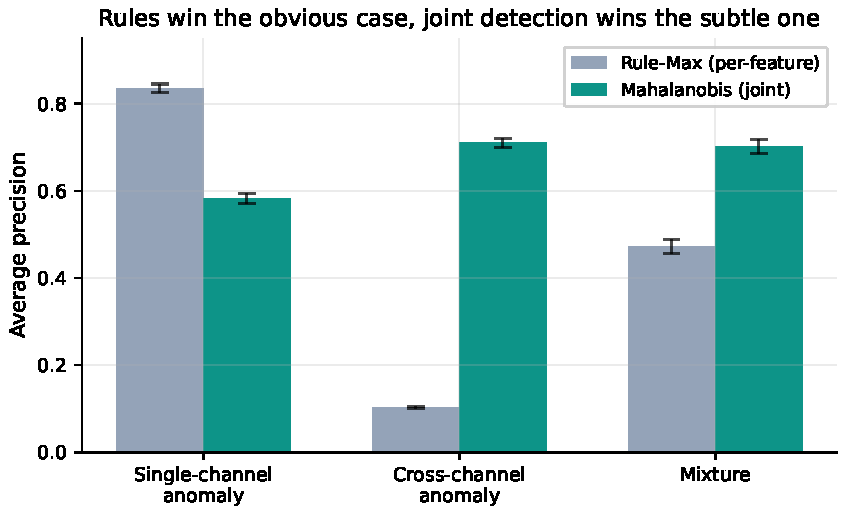
\includegraphics[width=\columnwidth]{fig1_crossover.pdf}
\caption{Per-feature rules win on single-channel anomalies; joint detection wins on cross-channel
anomalies and on the mixture.\\[2pt]\textit{Alt text:} Grouped bar chart with average precision on
the vertical axis and three anomaly conditions on the horizontal axis (single-channel, cross-channel,
and mixture), each showing a Rule-Max bar beside a Mahalanobis bar with error bars. Rule-Max is taller
on single-channel (about 0.84 versus 0.58), Mahalanobis is taller on cross-channel (about 0.71 versus
0.10), and Mahalanobis leads on the mixture (about 0.70 versus 0.47).}\label{fig:crossover}\end{figure}

\begin{figure}[t]\centering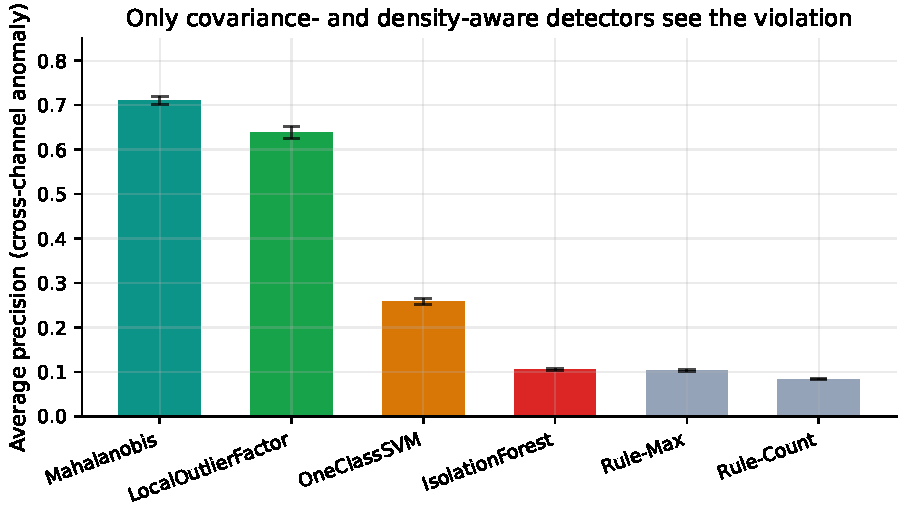
\includegraphics[width=\columnwidth]{fig2_detectors_cda.pdf}
\caption{On cross-channel anomalies, only covariance- and density-aware detectors see the
correlation violation; the axis-aligned Isolation Forest and the per-feature rules do not.\\[2pt]\textit{Alt text:}
Bar chart of cross-channel average precision (vertical axis) for six detectors (horizontal axis) with
error bars, ordered from highest to lowest: Mahalanobis (about 0.71), Local Outlier Factor (about
0.64), One-Class SVM (about 0.26), Isolation Forest (about 0.10), Rule-Max (about 0.10), and Rule-Count
(about 0.08). The first two bars are far taller than the remaining four, which sit near the prevalence
floor.}
\label{fig:detectors}\end{figure}

\section{Robustness and Sensitivity}
\label{sec:robustness}
The headline comparisons in Table~\ref{tab:ap} pit the single best detector against the single best
rule. To check that the conclusion is robust to which detector and which condition one looks at, we
report the margin of each joint detector over the \emph{best rule} in each condition, where the best
rule is the larger of Rule-Max and Rule-Count. The margin is the operationally meaningful quantity: it
is what a team gains, in average precision, by adding the joint detector on top of the rule layer it
already runs. Table~\ref{tab:margin} collects these margins, computed directly from the cell means of
Table~\ref{tab:ap}.

\begin{table}[t]
\centering
\caption{Average-precision margin of each joint detector over the best per-feature rule, by
condition. The best rule is Rule-Max on every condition (Single $0.836$, Cross $0.103$, Mixture
$0.473$). Positive values favor the joint detector; negative values favor the rule.}
\label{tab:margin}
\footnotesize
\setlength{\tabcolsep}{4pt}
\begin{tabular}{@{}lccc@{}}
\toprule
Joint detector & Single & Cross & Mixture \\
\midrule
Mahalanobis          & $-0.253$ & $\mathbf{+0.607}$ & $\mathbf{+0.229}$ \\
Local Outlier Factor & $-0.464$ & $+0.535$ & $+0.187$ \\
One-Class SVM        & $-0.289$ & $+0.156$ & $+0.056$ \\
Isolation Forest     & $-0.096$ & $+0.002$ & $-0.065$ \\
\bottomrule
\end{tabular}
\end{table}

The margin table sharpens three readings of the main result. First, the sign of the margin flips with
the condition for the covariance- and density-aware detectors: both Mahalanobis and Local Outlier
Factor trail the rule on single-channel anomalies (margins $-0.253$ and $-0.464$) and lead it on
cross-channel anomalies (margins $+0.607$ and $+0.535$), which is the conditional structure the study
set out to establish, now visible across the whole detector set rather than at a single cell. Second,
the Isolation Forest is the outlier among the joint detectors: its cross-channel margin is $+0.002$,
effectively zero, and its mixture margin is negative ($-0.065$), so on no condition does it earn its
place over the rule. An axis-aligned splitter is, by the floor argument of
Section~\ref{sec:theory}, the joint detector that behaves most like a rule. Third, the mixture column
is positive for the three coordinate-coupling detectors and negative only for the Isolation Forest,
confirming that the realistic mixed case still rewards a covariance- or density-aware second tier, at
a margin between the single-channel and cross-channel extremes.

\subsection{Adversarial reading: the correlation-only evasion}
The cross-channel anomaly is not only a model of accidental misconfiguration; it is the exact shape of
a deliberate evasion. Consider an adversary who has compromised a host and knows the defender monitors
it with per-feature threshold rules and, possibly, an off-the-shelf axis-aligned detector. The
adversary's goal is to keep the host's telemetry vector below every alarm while operating. The cheapest
way to do this is to hold each feature within its normal band: keep privileged-logon counts, unsigned-
binary fractions, and patch-debt figures each individually plausible, never crossing a threshold. An
adversary who succeeds at this has, by construction, produced a host whose marginals are normal but
whose joint structure need no longer respect the within-channel correlation that benign operation
imposes, which is precisely the cross-dimension anomaly of Section~\ref{sec:theory}. By
equation~(\ref{eq:Tequal}) such a host is invisible to every per-feature rule: Rule-Max and Rule-Count
sit at the prevalence floor ($0.103$ and $0.084$) against this evasion because the evasion was defined
to keep each marginal normal. By the box-mass argument of Section~\ref{sec:theory} it is equally
invisible to an axis-aligned Isolation Forest ($0.105$), which partitions on single coordinates and so
cannot condition on the cross term the evasion disturbs. The adversary thus defeats the entire
rule-based and axis-aligned monitoring stack with an evasion that costs only the discipline of staying
within per-feature norms. The covariance-aware detector is the monitor that closes this gap: it scores
the host by $x^{\top}\Sigma^{-1} x$, whose expectation~(\ref{eq:maha_gap}) is raised by exactly the
off-diagonal terms the evasion can no longer satisfy, and it reaches $0.710$ on this anomaly class
against the floor that the rules and the Isolation Forest occupy. The two-tier monitor is therefore not
only an accuracy improvement on benign misconfiguration but a closure of a concrete evasion channel: an
adversary who must keep every marginal normal still cannot keep the joint covariance normal, and the
covariance-aware tier is the one that holds them to it. The threat we do not close is an adversary who
can also forge the correlation structure itself, reproducing the within-channel covariance while
hiding malicious activity; that requires controlling the joint distribution of the telemetry, a
strictly harder attack than holding each marginal in band, and we note it as the residual threat the
present monitor leaves open.

\section{Discussion}
The question is not whether to use anomaly detection but which method to use and for which anomaly,
and the results give a clean answer. The two anomaly types call for two different tools, and the
mistake an operations team is most likely to make is to treat them the same.

Per-feature rules are the correct tool for single-channel anomalies. On the SDA condition Rule-Max
reaches 0.836 and beats every joint detector, including the best of them by 0.0954 with an interval
entirely below zero. A rule is cheap, auditable, and explainable to an authorizing official, and it
loses nothing to a joint detector on the anomalies it was built for. There is no case for replacing
rules on the obvious single-channel spikes; doing so adds machinery and removes interpretability for
no gain.

Joint detection is decisively better only for cross-channel anomalies, the subtle compromise-like
cases in which every signal is individually plausible but the host is jointly wrong. Here the best
joint detector reaches 0.710 against 0.103 for the best rule, a 0.607 gap, and the structure-blind
Rule-Count confirms that the gain comes from joint modeling rather than from aggregating marginal
alarms: counting exceedances reaches only 0.084. This is the case that justifies the cost of a joint
detector, and it is precisely the case a rule cannot reach.

Within joint detection, the standard advice to reach for an Isolation Forest is misleading for this
anomaly class. Its axis-aligned random splits cannot represent a correlation violation that leaves
every marginal normal, and it reaches only 0.105 on the cross-channel condition, no better than the
rules it was supposed to improve on. The detectors that work are the ones whose geometry is
disturbed by a broken covariance: the covariance-aware Mahalanobis (0.710) and the density-aware
Local Outlier Factor (0.638). The lesson generalizes beyond this study: the right base detector is
the one whose inductive bias matches the structure of the anomaly, and for a correlation violation
that means a covariance- or density-aware method, not an axis-aligned one.

The deployable recommendation is a two-tier monitor. The first tier is the per-feature rules already
in place, which catch the obvious single-channel spikes cheaply and remain the best tool for them.
The second tier is a covariance- or density-aware joint detector that runs alongside the rules and
catches the subtle cross-channel violations the rules miss. On the realistic mixture both tiers earn
their place: the joint detector leads (0.702 against 0.473), but by a smaller margin than on
cross-channel anomalies alone, because the rules are still carrying the single-channel half. The two
tiers are complementary, not competing, and a monitor that runs both covers both anomaly geometries
at the cost of one cheap rule layer and one well-chosen joint detector.

\section{Threats to Validity}
\emph{Construct validity.} The cross-channel anomaly is defined by a specific synthetic mechanism, a
within-channel correlation of $0.70$ in normal hosts that is set to zero in anomalous ones. Real
compromise telemetry may break correlation structure in other ways, by inducing spurious
cross-channel correlation rather than destroying within-channel correlation, or by shifting both
marginals and structure at once. The structural finding, that a correlation violation is invisible
to per-feature inspection and visible to a covariance- or density-aware detector, follows from the
geometry and should hold for any covariance violation, but the specific magnitudes depend on this
mechanism. The single-channel shift of $3.0$ standard deviations and the $8\%$ prevalence are
likewise documented priors rather than measurements.

\emph{Internal validity.} The detector hyperparameters are fixed at library defaults and are not
tuned on any seed (Isolation Forest 200 trees, One-Class SVM RBF with $\nu = 0.1$, Local Outlier
Factor 20 neighbors). This is conservative for the joint detectors, since tuning could only raise
their scores, but it means the absolute numbers for any one joint detector are untuned-default
values rather than best-achievable ones. A tuned Isolation Forest might do better on the
cross-channel case, though its axis-aligned construction limits how much; the comparative ordering
among the joint families reflects their inductive biases, not a tuning artifact. Because the study
is pre-registered and the evaluation seeds were inspected only once, the reported numbers are not the
product of analytic search.

\emph{Dimensionality and generalizability.} The hygiene vector has twelve dimensions in three
channels of four features each. Higher-dimensional telemetry, more channels, or a different
within-channel structure could change the absolute average-precision values and could affect the
density-based detector in particular, since local-density estimates degrade as dimensionality grows.
The fleet size of 1{,}500 hosts and the single-snapshot framing also abstract away temporal
structure that a real monitor would exploit. We expect the qualitative finding, that joint modeling
is needed for joint anomalies and that the right joint method is covariance- or density-aware, to
transfer, because it rests on the geometry of the anomaly rather than on the specific constants, but
absolute values should be read as illustrative of the model rather than as field estimates.

\emph{Statistical validity.} Intervals are BCa bootstrap intervals over 25 seeds with 10{,}000
resamples~\cite{efron1987bca,efron1994introduction}, appropriate for the small-sample, possibly
skewed average-precision differences reported here. We use interval non-overlap as the evidentiary
standard throughout rather than significance testing, which avoids the multiple-comparison hazards of
repeated $p$-values across detectors and conditions~\cite{wohlin2012experimentation}. Twenty-five
seeds is a modest sample, but the cross-channel intervals are narrow and far from their thresholds,
so the qualitative verdicts are not on the edge of significance.

\section{Conclusion}
Whether multivariate machine-learning anomaly detection earns its complexity over per-signal
threshold rules has a conditional answer that depends on the geometry of the anomaly. On
single-channel anomalies, the obvious threshold-crossing spikes, a per-feature rule wins (Rule-Max
0.836) and no joint detector improves on it, so the rule should stay. On cross-channel anomalies, the
subtle compromise-like cases where every signal is individually normal but the correlation structure
is broken, a joint detector is decisively better (Mahalanobis 0.710 against 0.103 for the best rule,
difference 0.607), and the gain requires joint modeling rather than aggregation, since a
structure-blind exceedance count reaches only 0.084. The choice of joint method is itself decisive:
covariance-aware and density-aware detectors see the violation (Mahalanobis 0.710, Local Outlier
Factor 0.638) while the popular axis-aligned Isolation Forest does not (0.105), so it is the wrong
default for this anomaly class. On a realistic fifty-fifty mixture the joint detector still leads
(0.702 against 0.473) but by a smaller margin (0.2285), because the rules still carry the
single-channel half. The deployable guidance is a two-tier monitor: keep cheap per-feature rules for
the obvious single-channel spikes and add a covariance- or density-aware detector for the subtle
cross-channel violations. Validating the synthetic correlation model against real compromise
telemetry is the natural next step toward turning these structural findings into field estimates.

\section*{Data Availability Statement}
The data and code that support the findings of this study are openly available in the research-papers repository at \url{https://github.com/Harshavardhanmalla-Labs/research-papers/tree/main/paper16}. The manuscript sources, figures, analysis code, and frozen result tables are included and regenerate every reported number deterministically from the fixed seeds.

\section*{Disclosure Statement}
No potential conflict of interest was reported by the author.

\section*{Funding}
No funding was received.

% Generated by IEEEtran.bst, version: 1.14 (2015/08/26)
\begin{thebibliography}{10}
\providecommand{\url}[1]{#1}
\csname url@samestyle\endcsname
\providecommand{\newblock}{\relax}
\providecommand{\bibinfo}[2]{#2}
\providecommand{\BIBentrySTDinterwordspacing}{\spaceskip=0pt\relax}
\providecommand{\BIBentryALTinterwordstretchfactor}{4}
\providecommand{\BIBentryALTinterwordspacing}{\spaceskip=\fontdimen2\font plus
\BIBentryALTinterwordstretchfactor\fontdimen3\font minus
  \fontdimen4\font\relax}
\providecommand{\BIBforeignlanguage}[2]{{%
\expandafter\ifx\csname l@#1\endcsname\relax
\typeout{** WARNING: IEEEtran.bst: No hyphenation pattern has been}%
\typeout{** loaded for the language `#1'. Using the pattern for}%
\typeout{** the default language instead.}%
\else
\language=\csname l@#1\endcsname
\fi
#2}}
\providecommand{\BIBdecl}{\relax}
\BIBdecl

\bibitem{cisakev}
{Cybersecurity and Infrastructure Security Agency (CISA)}, ``Known exploited
  vulnerabilities catalog,''
  \url{https://www.cisa.gov/known-exploited-vulnerabilities-catalog}, 2026.

\bibitem{chandola2009anomaly}
V.~Chandola, A.~Banerjee, and V.~Kumar, ``Anomaly detection: A survey,''
  \emph{ACM Computing Surveys}, vol.~41, no.~3, pp. 1-58, 2009.

\bibitem{hodge2004survey}
V.~J. Hodge and J.~Austin, ``A survey of outlier detection methodologies,''
  \emph{Artificial Intelligence Review}, vol.~22, no.~2, pp. 85-126, 2004.

\bibitem{davis2006pr}
J.~Davis and M.~Goadrich, ``The relationship between precision-recall and {ROC}
  curves,'' in \emph{Proceedings of the 23rd International Conference on
  Machine Learning}, 2006, pp. 233-240.

\bibitem{efron1987bca}
B.~Efron, ``Better bootstrap confidence intervals,'' \emph{Journal of the
  American Statistical Association}, vol.~82, no. 397, pp. 171-185, 1987.

\bibitem{efron1994introduction}
B.~Efron and R.~J. Tibshirani, \emph{An Introduction to the Bootstrap}.\hskip
  1em plus 0.5em minus 0.4em\relax Chapman \& Hall/CRC, 1994.

\bibitem{wohlin2012experimentation}
C.~Wohlin, P.~Runeson, M.~H{\"o}st, M.~C. Ohlsson, B.~Regnell, and
  A.~Wessl{\'e}n, \emph{Experimentation in Software Engineering}.\hskip 1em
  plus 0.5em minus 0.4em\relax Springer, 2012.

\bibitem{breunig2000lof}
M.~M. Breunig, H.-P. Kriegel, R.~T. Ng, and J.~Sander, ``{LOF}: Identifying
  density-based local outliers,'' in \emph{Proceedings of the 2000 ACM SIGMOD
  International Conference on Management of Data}, 2000, pp. 93-104.

\bibitem{scholkopf2001oneclass}
B.~Sch{\"o}lkopf, J.~C. Platt, J.~Shawe-Taylor, A.~J. Smola, and R.~C.
  Williamson, ``Estimating the support of a high-dimensional distribution,''
  \emph{Neural Computation}, vol.~13, no.~7, pp. 1443-1471, 2001.

\bibitem{liu2008isolation}
F.~T. Liu, K.~M. Ting, and Z.-H. Zhou, ``Isolation forest,'' in \emph{2008
  Eighth IEEE International Conference on Data Mining}, 2008, pp. 413-422.

\bibitem{aggarwal2015outlier}
C.~C. Aggarwal and S.~Sathe, ``Theoretical foundations and algorithms for
  outlier ensembles,'' \emph{{ACM} {SIGKDD} Explorations Newsletter}, vol.~17,
  no.~1, pp. 24-47, 2015.

\bibitem{rousseeuw1999mcd}
P.~J. Rousseeuw and K.~Van~Driessen, ``A fast algorithm for the minimum
  covariance determinant estimator,'' \emph{Technometrics}, vol.~41, no.~3, pp.
  212-223, 1999.

\bibitem{fips199}
{National Institute of Standards and Technology}, ``Standards for security
  categorization of federal information and information systems,'' U.S.
  Department of Commerce, Tech. Rep. FIPS PUB 199, 2004.

\bibitem{nist80053}
{Joint Task Force}, ``Security and privacy controls for information systems and
  organizations,'' National Institute of Standards and Technology, Tech. Rep.
  NIST Special Publication 800-53 Rev. 5, 2020.

\bibitem{nist80137}
K.~Dempsey, N.~S. Chawla, A.~Johnson, R.~Johnston, A.~C. Jones, A.~Orebaugh,
  M.~Scholl, and K.~Stine, ``Information security continuous monitoring (iscm)
  for federal information systems and organizations,'' National Institute of
  Standards and Technology, Tech. Rep. NIST Special Publication 800-137, 2011.

\bibitem{cjis2023}
{Federal Bureau of Investigation}, ``Criminal justice information services
  (cjis) security policy, version 5.9.2,''
  \url{https://www.fbi.gov/file-repository/cjis-security-policy-v5-9-2-20221207.pdf},
  2022.

\bibitem{paper3hygienebench}
H.~Malla, ``{HygieneBench}: A reproducible synthetic benchmark for
  cyber-hygiene anomaly detection across identity, endpoint, and patch
  telemetry,''
  \url{https://github.com/Harshavardhanmalla-Labs/research-papers/tree/main/paper3},
  2026, companion paper; source, code, and frozen results in the same
  repository.

\bibitem{paper4hygieneprio}
H.~Malla, ``{HygienePrio}: Cyber-hygiene signal augmentation for
  {EPSS}-weighted vulnerability prioritization,''
  \url{https://github.com/Harshavardhanmalla-Labs/research-papers/tree/main/paper4},
  2026, companion paper; source, code, and frozen results in the same
  repository.

\bibitem{cover2006elements}
T.~M. Cover and J.~A. Thomas, \emph{Elements of Information Theory},
  2nd~ed.\hskip 1em plus 0.5em minus 0.4em\relax Wiley, 2006.

\end{thebibliography}

\end{document}
